Inventory management, or storage management, can be qualified as the art of storing and ordering goods in a clever way with respect to some criteria (most often the cost). It can be applied at both the beginning and the end of the production system (even in between actually). At the beginning of this chain, raw materials are delivered by the suppliers and are stored in a warehouse. The storage is emptied when the production site requires some raw materials to be used for production. On the other side of the chain, at the end, the storage is filled with final products and is emptied by the market demand. Though the two situation may appear different in some kind, we can jointly study them considering some sort of "abstract demand" (either production demand or market demand) and some sort of "abstract supplier" (either a real supplier which provides raw material or the production site itself). See figure (\ref{continuous:storage}) for graphical representation.

\begin{figure}[h!]
    \centering
    \begin{tikzpicture}[scale=0.8]
        \draw (-2, .5) node [left] {supplier};
        \draw (7, .5) node [right] {demand};
        \draw (2.5, -3) node [below] {storage};
        \draw (0,0) -| (0,-3) -| (5, 0);
        \draw[->] (-2, .5) -| (.5, -2);
        \draw[<-] (7, .5) -| (4.5, -2);
        \draw [decorate,decoration=snake] (0,-2.3) -- +(5,0);
    \end{tikzpicture}
    \caption{\label{continuous:storage}Storage management parameters}
\end{figure}

To study the inventory management, we introduce models that tend to represent real life cases. Making different assumptions on the demand and supplier, we end with different models. The simplest model is the so called "deterministic model" where all the input data for our problem are supposed to be perfectly known in advance (both the supply and the demand). We will start by studying this model before focusing on a "stochastic model" where the supplier and the demand are modeled by random variables. 

In this chapter, we will study what is called "continuous inventory management". What we mean by this is that the time is modeled by a continuous variable ($t\in\mathbb R$). In the next chapter, we'll deep into "periodic inventory management" where the time is modeled by a discrete variable ($t\in\mathbb N$). 

\section{Deterministic model}

The deterministic model supposes that we exactely know both the demand and the characteristics of our supplier. We denote by $\lambda$ the rate at which the storage is emptied. In the case where our warehouse is at the end of our chain, just after the production site, $\lambda$ represents how many items (final products) we sell by unit of time. If considered at the beginning of the chain, it corresponds to how many items (raw materials) are needed by our production site. This coefficient can be computed as \[ \lambda = \frac{\textrm{nb of items leaving the warehouse}}{\textrm{observed time}} \]

To fullfill that demand, we need to order a certain quantity of good, which will cost us some amount of money. In fact, the costs are of three kinds : 
\begin{itemize}
    \item A \textbf{fixed cost} which we have to pay for each order we make to our supplier. Let $K$ denote this cost, expressed as $euros/order$
    \item An \textbf{inventory cost} which we pay for storing goods in our warehouse, expressed as $euros/(time\times item)$. Let $h$ be the inventory cost.
    \item A \textbf{unitary cost} which corresponds to the price of each item per se. We will refer to this cost as $c$, expressed as $euros/item$
\end{itemize}

For sure, it is easy to see that choosing the right time and quantity to order goods is a matter of balancing between the fixed cost we pay for ordering an independent amount of product and the inventory cost which we pay for storing the goods. If storing products in our warehouse is very expensive for us, we might prefer to order often and pay the fixed cost multiple times rather than paying it just once and be left with a lot of goods we pay a fortune for storing. If, however, the inventory cost is very low (which means that we can store many items for a small amount of money), we'd rather order a lot of products and store them for a long time if needed. So, how do we compute the total cost ? 

Let $T$ be the period of time between the moment we order some goods and the moment our storage goes empty. Note that since the demand is deterministic and known in advance there is no risk of "unpredicted" events which could lead us to be unable to fullill the demand nor to order too many items in such a way that some would remain after some time. Finally, let $Q$ be the number of items we will buy at the beginning of that period. The figure (\ref{continuous:triangles}) sums up some of the introduced variables. 

\begin{figure}[h!]
    \centering
    \begin{tikzpicture}[scale=0.8]
        \draw[<->] (0, 5) node (yaxis) [above] {$I(t)$} |-  (10, 0) node (xaxis) [below] {$t$};

        \draw (.5, 0) -- ++(0, 4) -- ++(3.5, -4) -- ++(0, 4) -- ++(3.5, -4);
        \draw (8, 1) node {...};
        \draw[dotted] (0, 4) node [left] {$Q$} -- (7,4);
        \draw (2.5, 2.5) node {$-\lambda$} ++(3.5, 0) node {$-\lambda$};
        \draw[<->] (.5, -.5) -- (4, -.5);
        \draw (2, -1) node {$T$};

    \end{tikzpicture}
    \caption{\label{continuous:triangles}Inventory level in the deterministic model}
\end{figure}

For a given period of time $T$, we can then compute the total cost as
    \[ J_T = 
        \underbrace{\vphantom{\int}K}_{\textrm{fixed cost}}
        +
        \underbrace{\vphantom{\int}cQ}_{\textrm{price for }Q\textrm{ items}}
        +
        \underbrace{\int_0^T hI(t)dt}_\textrm{storage cost}
    \]
where the integrated part is simply given by $\frac{QT}{2}$ (area of a triangle\footnote{$\int_0^ThIt(t)dt = \int_0^T h\times (Q-\lambda t) dt = h[Qt-\lambda \frac{t^2}2 ]_0^T = h\frac{2QT-\lambda T^2}{2}$ and since $Q=\lambda T$ we get $\frac{QT}{2}$ by substituting $\lambda$}). 

For sure, we want to minimize the cost for a given period of time. That cost is given by \[ J = \frac{1}{T}\left( K + cQ + \frac{hQT}{2} \right) = \frac{K\lambda}Q + c\lambda + \frac{hQ}{2} \]
Note that we used the fact that $Q = \lambda T$ holds. Regarded as a function of $Q$, we can analyse its variations by derivation (since $Q=0$ does not make any sense for our purpose, it is for sure differentiable) : 
\[
    \begin{cases}
        \frac{dJ}{dQ} &= -\frac{K\lambda}{Q^2} + \frac{h}{2} \\
        \frac{d^2J}{dQ^2} &= \frac{K\lambda}{Q^3}
    \end{cases}
\]

Solving the optimality condition $\frac{dJ}{dQ} = 0$ we get that \[Q^* = \sqrt{ \frac{2K\lambda}{h} } \] can be regarded as a critical point of $J$. And, since the second derivative of $J$ is positive, the value $Q^*$ corresponds to a minimum of our cost function. This quantity is known as the \textbf{Economic Order Quantity} (EOQ) and corresponds to the number of items we should order every $Q/\lambda$ unit of time in order to minimize the total cost. 

We may discuss the obtained formula noting that : (1) if the fixed price for order is very large with respect to the inventory cost, we will by a large amount in once and store it for a long period of time ; (2) if the demand is high, we buy more ; (3) if the inventory cost is large with respect to the fixed cost per order, we will prefer making multiple orders in order to store as less as possible. 

The moment at which we should order that quantity $Q^*$ of goods is given by the characteristics of our supplier. Let $\tau$ be the lead-time of our supplier (difference between the moment we make an order and the moment we actually recieve the products). We define the so called \textbf{reorder point} as $R = \lambda\tau$ which corresponds to the inventory level at which we should call the supplier to make an order\footnote{Note that in the deterministic case, directely using the lead-time is strictly equivalent to using the reorder point, however, three arguments to use the re-order point rather than the lead-time : (1) the reorder point is linked to a quantity that the warehouse can directly control, (2) the deterministic case is a model, which can or can not reflect the reality, using the reorder point assures us that if, for unexpected reasons, we get to the reorder point sooner than planned, we can still make an order at the right time for the new period of time, (3) we will keep using that quantity in the stochastic case.}.

\section{Stochastic model}

In the previous model, we supposed that we could both know perfectly the demand and the lead-time of our supplier. In real life however, such quantities are often subject to variations and are found by estimation. That being said, we can not afford to trust a deterministic formula since we know that life is full of unpredicted and unpredicatable events. Let $x$ be a random variable such that $x\sim\mathcal N(0,1)$. We now model the demand (denoted $d$ by convention in the stochastic model) by a random variable given by $d=\bar d + \sigma_d x$ and the lead-time by $\tau = \bar\tau +\sigma_\tau x$. 

Actually, the stochastic model is a generalisation of the deterministic model and a lot of common aspects will remain true in this model (in the sense that we can derive the deterministic case from the stochastic case). But, since the demand now variates with time, we can no longer rely on an exact formula giving us \emph{exactely} how many goods we have to order in order to have a $0$-inventory-level when we re-order some other goods. Instead, we'd rather save some goods to prevent the fact of being short on stock. That amount of goods is called the \textbf{safety stock} and will be denoted by the variable $s.stock$. Given these informations, what is reasonnable to expect ? 

The expected value of the demand (resp. the leadtime) is $\bar d$ (resp. $\tau$). The reorder point is thus expected to be given by $\bar d\bar\tau$ which, in average, would bring the inventory level to $0$ before re-ordering. To this quantity, we add the safety stock to prevent us from delays of our supplier. \[ R = \bar d\bar \tau + s.stock \] In average, the stochastic model should be exactely the deterministic model shifted up by precisely $s.stock$ goods in the inventory. The figure (\ref{continuous:realisations}) represents two realisations of the demand while figure (\ref{continuous:average}) represents the expected value of our inventory level. 

\begin{figure}[h!]
    \centering
    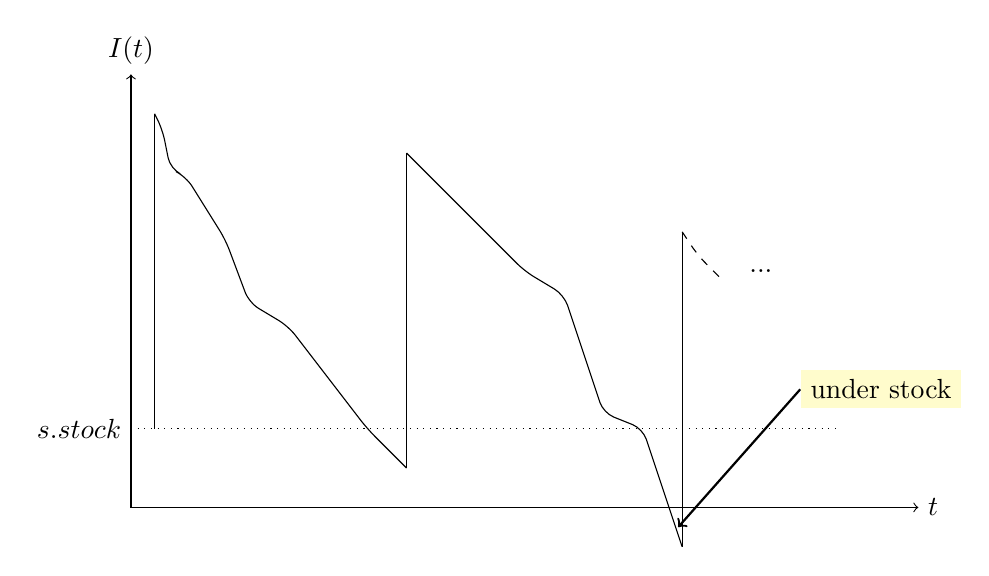
\begin{tikzpicture}
        \draw[<->] (0, 5.5) node [above] {$I(t)$} |- (10, 0) node [right] {$t$};
        \draw[dotted] (0, 1) node [left] {$s.stock$} -- (9, 1);
        \draw (.3, 1) -- (.3, 5);
        \draw[rounded corners] (.3, 5) -- (.4, 4.8) -- (.5, 4.3) -- (.7, 4.2) -- (1.2, 3.4) -- (1.5, 2.6) -- (2, 2.3) -- (3, 1) -- (3.5, .5);
        \draw (3.5, .5) -- (3.5, 4.5);
        \draw[rounded corners] (3.5, 4.5) -- (5, 3) -- (5.5, 2.7) -- (6, 1.2) -- (6.5, 1) -- (7, -.5);
        \draw (7, -.5) -- (7, 3.5);
        \draw[rounded corners, dashed] (7, 3.5) -- (7.2, 3.2) -- (7.5, 2.9);
        \draw (8, 3) node {...};
        \draw[<-, thick] (6.95, -.25) -- (8.5, 1.5) node [right, fill=yellow!20] {under stock};
        
    \end{tikzpicture}
    \caption{\label{continuous:realisations}Two realisations of the demand}
    \begin{tikzpicture}
        \draw[<->] (0, 5.5) node [above] {$\mathbb EI(t)$} |- (10, 0) node [right] {$t$};
        \draw (.3, 1) -- ++(0, 4) -- ++(3.5, -4) -- ++ (0, 4) -- ++(3.5, -4);
        \draw[dotted] (0, 5) node [left] {$Q$} -- (9, 5);
        \draw (2, 3.5) node {$-\bar d$} ++(3.5, 0) node {$-\bar d$};
        \draw[dotted] (0, 1) node [left] {$s.stock$} -- (9, 1);
        \draw (8, 3) node {...};
    \end{tikzpicture}
    \caption{\label{continuous:average}Expected inventory level}
\end{figure}

The expression of the cost must now be updated since we no longer only pay for ordering and storing the goods which are used to fulfill the demand but also for storing some goods as a safety-stock. The total cost is now given by : 

\[ J = \frac{K\bar d}{Q} + c\bar d + \frac{hQ}{2} + h\times s.stock \]

This function of two variables ($Q$ and $s.stock$) is actually well splittable into two functions of one variable denoted by $f(Q)$ and $Q(s.stock)$. It is clear that minimizing the total cost can now be done by minimizing both functions seperately. Regarding the first function $f$, the computations remains the same as in the previous section (deterministic model) and we still have $Q^* = \sqrt{2K\bar d}{h}$. Minimizing $g$ how ever, requires some more analysis. Of course, $g$ is linear with respect to $s.stock$ so the global minimum is $0$ since it cannot be negative. But setting it to $0$ would mean risking to be short on stock at some point. We, somehow, want to control the risks we take and two strategies can be opted for :

\begin{enumerate}
    \item Let $d_\tau$ be the demand over the lead-time $\tau$. It is clear that $d_\tau$ is \emph{linked} to both $d$ and $\tau$ but it is a rather strong assemption to say that these two random variables are \emph{dependent}. Indeed, the realisation of the leadtime of a supplier is not dependent on the global demand\footnote{it is surely linked, for example, during peak demands of a given good, one supplier may have difficulties to satisfy all of his clients, but we cannot consider that a truck getting lost, or breaking down depends on the demand}. $d_\tau$ is thus given by $d_\tau = \bar d_\tau + \sigma_{d_\tau}x $ where $\bar d_\tau = \bar d\bar\tau$ and $\sigma_{d_\tau}=\sqrt{ \sigma_d^2\bar\tau + \sigma_\tau^2\bar d^2 }$. One idea to select effectively the safety stock is to make sure that the probability of being short on stock is lesser than a certain number which we control. Being short on stock is realised when the demand over the lead-time is greater than the reorder point we have choosen. This strategy implies choosing $s.stock$ so that \[ \mathbb P(d_\tau\le R)\ge\alpha = \mathbb P\left(x\le\frac{R-\bar d_\tau}{\sigma_{d_\tau}}\right)\ge\alpha \] where $\alpha$ is called the "fill rate". 
    Using this strategy can be done as follow : 
    \begin{enumerate}
        \item Choose an acceptable probability $\alpha$
        \item Solve the eqution for $X$ and let $\bar X$ be the solution
        \item Subsitute $X$ by $\bar X$ in $s.stock = \bar d_\tau + \sigma_{d_\tau}X$
    \end{enumerate}
    \item As it has been previously said, it holds that we are short on stock when $d_\tau > R$ (more demand during the lead-time than the reorder point). Let $n(R)$ be the average number of unused items (items remaining in the warehouse when we re-order again).  We can compute this quantity with the following formula\footnote{For any random variable $X$ with density function $f$, the average value of $X$ is given by $\int_0^\infty xf(x)dx$} : \[ n(R) = \int_R^\infty (d_\tau-R)f(d_\tau)d(d_\tau) \] However, it is analytically hard to compute. To deal with that problem, we introduce the function $L$ which is called the loss function expressed as \[ L(X) = \int_X^\infty(t-X)f(t)dt\textrm{ where }f\textrm{ is the density of the normal law }\mathcal N(0,1) \] so that \[ n(R) = \sigma_{d_\tau}L(X) \] Finally, by defining the average percentage of unused items with respect to the total number of goods we buy, denoting it by $\beta=\frac{n(R)}{Q^*}$ we can find $s.stock$ so that \[ L(X) = \frac{\beta Q^*}{\sigma_{d_\tau}} \] where $\beta$ should of course be defined \emph{a priori} depending of the market requirements, of course, the lowest $\beta$ is, the greatest is the service.

    Using this second strategy can be done like so :
    \begin{enumerate}
        \item Compute $\sigma_{d_\tau}$
        \item Compute $\frac{\beta Q^*}{\sigma_{d_\tau}}$ and use the table to find the corresponding $X$ denoted $\bar X$
        \item Subsitute $X$ by $\bar X$ in $s.stock = \bar d_\tau + \sigma_{d_\tau}X$
    \end{enumerate}
\end{enumerate}